\chapter{Konzeption}

Im Kapitel {\em Konzeption} beginnt jetzt die Darstellung der eigenen Arbeit. Dieses Kapitel stellt das Bindeglied zwischen Zielsetzung, Stand der Forschung und der eigentlichen Umsetzung dar. Zusammen mit Implementierung und Evaluation macht die Konzeption den Hauptteil der Arbeit aus.

Typischer Umfang der Konzeption: 5-10 Seiten BA, 15-20 Seiten MA.

\section{Erstellung eines Unterrichts}
Die VR Übung ist eine ergänzige Lernmethode für das Lernen. Vor der Durchführung der Übung sollen genügendes Vorwissen angeboten werden. Deswegen wird erst einen Unterricht auf Learning Managment System erstellt.

Laut der Erklärung im Kapitel Stand der Forschung \glqq Multisensorische und emotionale Wahrnehmungen können die Gedächtnisleitung verstärken\grqq\ sollen die Lernmaterialien des Unterrichts vielfältig sein.  Durch drei Lernmateriallien werden das Vorwissen geboten:
\begin{enumerate}
    \item Text: Text ist das traditionelle Lernmaterial. Es spielt eine unersetzbare Rolle für Lernen. Die Lesegeschwindigkeit kann der Lernende sich selbst entscheiden. Während des Lesens kann der Leser gut denken, merken und notieren.
    \item Video: Video ist ein intuitives Lernmaterial. Zwei Wahrnehmungen, Sehen und Hören werden aufgerufen, wenn man Video anschaut. Durch Video kann die Handlung sehr konkret gezeigt. Zur Zeit ist Video das beste und verbreitete Medium, praktische Kenntnisse zu vermitteln.
    \item Diagramm: Diagramm ist eine optimale Darstellung für Struktur und Sequenz. Die deutliche visuelle Zeichnungen sind hilfreich für das Verständnis und Gedächtnis.
\end{enumerate}

Nach der Sammlung der Vorkenntnisse geht der Lernende durch die Zugang in diesem Unterricht in VR Umgebung rein, und wird die praktische Übung durchgeführt. In der Übung steht das Vorwissen als Hinweise zu Verfügung. Die Hinweise müssen nicht zwingend angeschaut werden, wenn der Lernende die Übung flüssig schaffen kann. Allerdings soll die Hinweise einfach erreichbar sein. Sodass muss der Lernende nicht aus VR Umgebung ausgehen, um Hilfsmittel zu suchen, wenn der Lernende nicht an der Vorkenntnisse erinnern kann. Wenn die Übung geschafft wird, wird der Lernende wieder zu dem Unterricht geleitet.

Nach der Übung wird ein Test geboten, um das Ergebnis des Lernens zu prüfen. Das Ergebnis des Tests wird in Learning Managment System gespeichert und als Feedback an dem Lehrende geschickt.

\section{WebVR}
Zwei Ziele des Projekts haben höchste Prioritäten: gute Erreichbarkeit und Verbindung mit LMS.

Der größte Vorteil der native Apps bei Erreichbarkeit ist offline Benutzbarkeit. Wenn die Applikation installiert ist, muss es während der VR Übung nicht online sein. Allerdings die Installation besitzt viele Kapazität von Rechner oder Smartphone. Wenn viele Übungen werden in eine Applikation eingepackt, führt es zu Missbrauch der Kapazität, weil tatsächlich die geschaffte Übungen nicht gebraucht sind. Wenn jede Übung eigne Applikation hat, wird viele extra Zeit in Installation vor dem Lernen investiert, deshalb existiert der Vorteil offline Erreichbarkeit nicht mehr.

Obwohl Web Apps das Internet gefordert, ist sie jede Zeit erreichbar ist.

Capterra ist eine Webseite, die deren Benutzer hilft, geeignet Software in unterschiedlichen Bereichen zu finden. Es werden insgesamt 432 Softwares gefunden, wenn \glqq LMS Software \grqq\ gesucht wird. 406 von 432 gefundene LMSs haben web basierte Applikation zu Verfügung. Das heißt, dass 94\% LMS können in Browser laufen lassen.

WebVR Applikation wird auch in Browser aufgerufen. Ohne software Wechseln wird zu keiner Ablenkung geführt. Außerdem ist die Schnittstelle zwischen Web Applikationen einfach zu implementieren.

Laut oben genannten Gründe wird für WebVR Technik entschieden, die VR Übung zu realisieren.

\section{Verbindung zwischen WebVR Applikation und Learning Managment System}
Es gibt drei Formen für die Verbindung zwischen WebVR Applikation und Learning Managment System(LMS):
\begin{enumerate}
    \item WebVR Applikation neben dem Learning Managment System:
     \subitem In LMS wird die Zugang zur VR Umgebung geboten und durch URL können Informationen in VR Umgebung eingefügt werden. In Vr Umgebung wird auch die Zugang zurück zu LMS geboten. Aber keine Information kann von VR Umgebung an LMS übermittelt werden.
     
     Der Vorteil ist, dass die WebVR Applikation unabhängig von LMS ist. Jede LMS kann mit der WebVR Applikation verbinden.
     
     Der Nachteil ist, dass der Umtausch der Informationen ziwischen WebVR Applikation und LMS einspurig ist. Das LMS kann Keine Information von WebVR Appliaktion bekommen. Außerdem wird jede Änderung in WebApp z.B. Umschreibung des Hinweises durch Programmierer gemacht. Der Lehrende ist nicht in der Lage, alleine die Übung zu verbessern oder korrigieren.
     
    \item WebVR Applikation teilweise in dem Learning Managment System:
     \subitem In LMS wird die Zugang zur VR Umgebung geboten, allerdings die Zugang nicht ein URL, sondern erfahrungsmäßig ein Plugin ist. Durch das Plugin kann die WebVR Applikation die versteckte zugängliche Daten der Datenbank des Unterrichts bekommen. Mit solche Daten ist die WebVR Applikation in der Lage, die Daten in Datenbank zu speichern und die Daten aus Datenbank zu lesen. Durch das Middleware wird die gegenseitige Kommunikation zwischen WebVR Applikation und LMS ermöglichen. Obwohl durch URL die zugängliche Daten auch übergetragen werden können, ist es sehr unsicher für das LMS.
     
     Der Vorteil ist, dass die Kommunikation zwischen WebVR Applikation und LMS frei ist. Das heißt, dass die übergetragene Daten nicht nur Parameter sondern auch Bilder, Audios und Videos sein können und das LMS kann die Informationen, die während der Übung in WebVR Applikation erstellt, bekommen. Darüber hinaus kann der Lehrende durch dem Plugin die Inhälte in WebVR Applikation direkt andern.
     
     Die Nachteile sind, dass die WebVR Applikation von dem LMS abhängig ist und die Entwicklung aufwendig ist. Um die Daten barrierefrei überzutragen, muss entsprechende Schnittstelle in WebVR Applikation konfiguriert werden. Bei der Entwicklung werden nicht nur WebVR Applikation, sondern auch das Plugin von LMS geschrieben. Zusätzlich wird eine Datenbank eingerichtet.
     
    \item Learning Management System in WebVR Applikation
     \subitem Bei dieser Form ist die Methode der Kommunikation zwischen WebVR Applikation und LMS gleich wie die zweite Form. Der größte Unterschied liegt an der Benutzererfahrung. Die Graphical User Interface(GUI) des LMSs wird in der VR Umgebung dargestellt. Das heißt, dass vom Anfang an der Lernende in der VR Umgebung steht. In der VR Umgebung wird Vorwissen gesammelt, praktische Übung durchgeführt und Test gemacht.
     
     Der Vorteil ist, dass der ganze Lernprozess in VR Umgebung integriert wird, keine Ablenkung existiert.
     
     Die Nachteile sind aufwendige Entwicklung und ungewöhnliche Erfahrung des Lesens.
\end{enumerate}
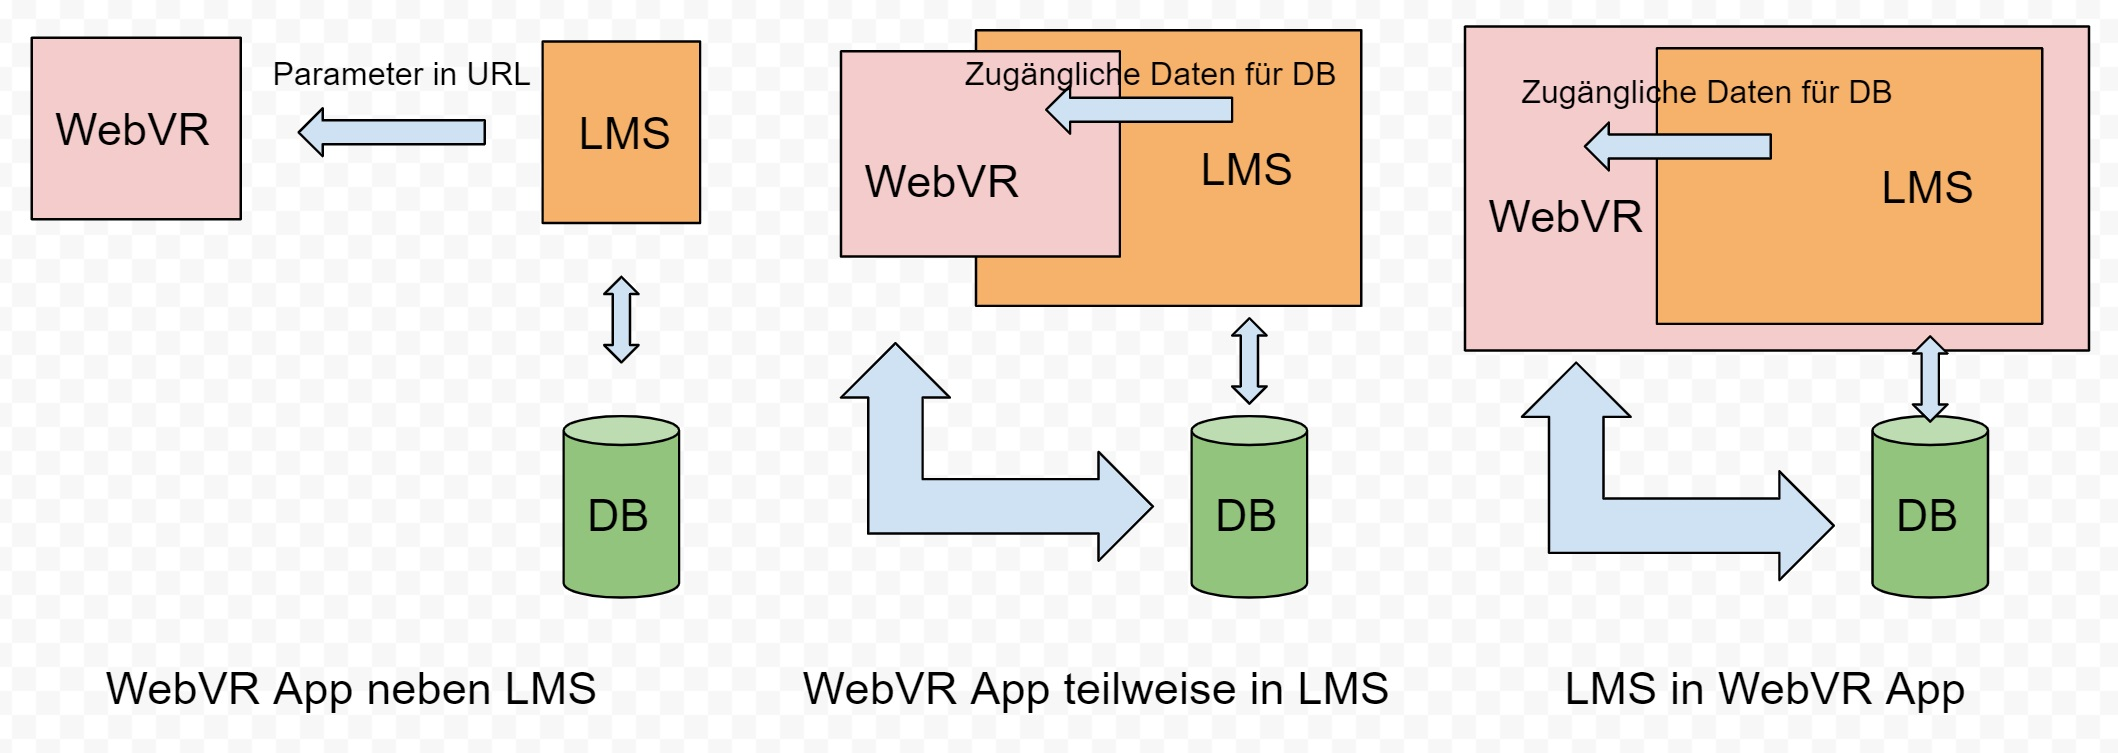
\includegraphics[width=\textwidth]{images/formenDerVerbindung.jpg}

Bei diesem Projekt wird erste Form implementiert. Wegen der begrenzte Entwicklungszeit werden die zweite und dritte Formen bei diesem Projekt nicht realisiert.

\section{Interaktion}
Interaktion ist der Hauptteil der WebVR Applikation, weil die nicht nur die Implementierung von Interactability von der Kategorie der Immersion ist, sonder auch enge Beziehung mit Matching hat. Da die WebVr Applikation cross-platform ist, werden die Konzeptionen der Interaktion nach den Typen der Geräte gliedert.

 \subsection{Desktop und Laptop}
  \subsubsection{Bewegung des Aspekts}
  Der Aspekt ist die Sicht, die in Kamera aufgenommen ist, nämlich die Sicht des Benutzers. Die Bewegung des Aspekts wird nach der Bewegung der Maus geführt. Es gibt zwei Varianten, um die Bewegung des Aspekts zu bestimmen.
  
  Eine Variante ist, dass die Bewegung des Aspekts aufgerufen wird, wenn die linke Taste der Maus gedrückt. Wenn die linke Taste losgelassen wird, bewegt sich der Aspekt nicht. Der Vorteil ist, dass solche Interaktion ähnlich wie alltägliche Applikation beispielsweise Google Map. Sodass wird die Interaktion schnell gewöhnt. Der Nachteil ist, dass eine Aktivität durch zwei Aktionen, Maus Druck und Maus Bewegung, aufgerufen werden. Das macht die Interaktion kompliziert, wenn der Aspekt sich häufig bewegt.
  
  Die andere Variante ist, dass die Bewegung Mode aktiviert wird. Das heißt, dass die Aspekt sich solange nach der Maus bewegt, bis ESC Taste gedrückt wird. Der Vorteil ist, dass die Interaktion einfach ist, und der Druck auf Maus verringert wird. Der Nachteil ist, dass der Mauszeiger während der Bewegung Mode verschwindet ist. Es könnte passiert, dass der Benutzer die Maus in einer großen Auswahl schwenkt, um den Mauszeiger zu finden, sodass der Aspekt auch schwer wackelt.
  
  Die verwirrende Aktivität bei zweite Variante passiert normalerweise nur bei der erst mal Nutzung und ist harmlos. Allerdings der Vorteil davon ist eindeutig. Deshalb wird die zweite Variante implementiert.
  
  \subsubsection{Bewegung der Kamera}
  Die Position der Kamera ist der Ort, wo der Benutzer in der VR Umgebung steht. Die Bewegung der Kamera ist die Bewegung des Benutzers.
  Zwei Möglichkeiten der Bewegung werden gebogen, eine zwingende und eine freiwillige.
  
  Zwingende Bewegung bedeutet, dass die Kamera sich automatisch zu einem Ort bewegt. Das Ziel ist, der Benutzer zu leiten, Objekten zu betrachten. Zum Beispiel soll die Plakate um die Desinfektion der Hände Während der Desinfektion richtig betrachtet werden, deswegen bewegt sich die Kamera zwingend zu der Plakate, wenn der Benutzer Hände desinfizieren will.

  Außer der zwingende Bewegung kann die Kamera durch die Taste W, A, S, D auf die Tastatur gerückt. Das bietet die Freiheit, die VR Umgebung sich umzuschauen. Ohne die freiwillige Bewegung der Kamera kann die Übung auch barrierefrei durchgeführt werden.
  
  \subsubsection{Zeiger} 
  Zeiger ist ein schwarzer Ring, der immer in der Mittel der Sicht der Kamera steht. Der ist zuständig für den Aufruf eine Aktivität eines Objekts. Wenn der Benutzer mit dem nächsten Objekt hinter dem Zeiger interagieren kann, wechselt der Farbe des Rings zu grün, um das Selbstvertrauen dem Benutzer zu geben, die Aktivität zu aktivieren. Wenn die linke Taste der Maus gedrückt wird, scheint die Farbe des Rings rot für ca. 0,3 Sekunde, um die Botschaft an dem Benutzer geben, dass der Befehl, mit einem Objekt zu interagieren, ausgeführt ist. 
  
 \subsection{Smartphone}
  \subsubsection{Bewegung des Aspekts}
  
\begin{itemize}
\item white board
\item Interaktion
\subitem flach Bildschirm: cursor, gaze
\subitem GearVR: gaze, click
\subitem HTC Vive: drag, press release, hand, check
\subitem observer patern
\item Töne
\item section selection: observerpatern
\item hand
\end{itemize}